%# -*- coding: utf-8-unix -*-
%%==================================================
%% chapter02.tex for SJTU Master Thesis
%% based on CASthesis
%% modified by wei.jianwen@gmail.com
%% Encoding: UTF-8
%%==================================================

\chapter{实验与分析}
\label{chap:experiment}




\section{实验设计}


\subsection{实验目的}
在进行我们主要的语言模型Multi-view架构测试与对比的实验之前,我们先将辅助的实验进行测试,选取,比较。

首先,我们想探究什么样的辅助信息可以被应用提升我们的模型。因为我们的架构的两部分的模型:标注模型和语言模型是以此层面链接在一起的,语音识别的过程中的语言模型也是以词为单位的,因为只考虑词层面的辅助特征,因为我们仅仅考虑词性标注(POS)、命名实体识别(NER)和语法块标注(CHUNK)等三种信息。在此基础上,我们需要完成并实现辅助信息标注的提取工具并进行测试和评估。

第二,根据前文所说的,我们架构中包含一个单向标注模型,而这个标注模型相比于当前应用比较多的双向标注模型之间的差距我们得测试清楚,需要确定采用单向标注是否会损失太多模型信息。为了测试这个模型,我们的训练数据采用斯坦福大学的标注工具作为真实标注,比较它们之间的差距。
其中斯坦福的工具为
Core-NLP tools\footnote{http://nlp.stanford.edu/software/}
后面也将以这个标注作为对比进行我们模型和其他模型的比较。

第三,由于实验架构中使用到了本人的另一个研究内容:前文详细描述过的$\beta$稳定算子自适应算法在LSTM语言模型中的应用。
因此我们将$\beta$稳定算子自适应算法在LSTM语言模型中的影响和效果,相比于普通的LSTM语言模型进行比较并得出最好的使用方法的结论。

第四,根据前文提到的五种对于本文模型架构的不同训练方法,由于我们没有那么多机器时间对所有的数据集都在五种方法上进行尝试和比较,因此我们仅在最小的中文短信数据集上对五种方式进行实验比较,最终得出效果最好的一种训练方式,并将这种方式用于所有其它数据集上的实验。

最后就是首先对本文提出的第一个单向辅助信息Multi-view语言模型和其它LSTM和Mulit-view语言模型以及Multi-task语言模型之间的比较。
比较实验主要在PPL和ASR重打分两个维度上展开。

结构在本文提出的第二个结构化语言模型——Teacher-student模型结构上的实验和对比。

实验部分在所有实验,无论是辅助实验还是主要结构化比较实验中,都一边给出实验参数、展示实验数据,一边进行分析和给出结论。


在所有的多视角语言模型实验和Teacher-student实验中,我们采取的都是单层LSTM语言模型,在学习率自适应的实验中我们会采取多层的模型进行验证。其中所有的隐层都是大小为300的LSTM结构,并且所有的模型都采用dropout比率为$0.5$的训练方法。如果有极少数的意外情况会在实验结果说明中提及。



\subsection{测试标准}

混淆度是一种常见的衡量自然语言处理领域(NLP)中的语言模型的好坏的指标,通俗的讲就是对于语言模型所估计的一句话出现的概率,用句子长度进行归一化。          
混淆度是由语言模型和测试句子之间的交叉熵算出来的,不同的测试句子测得的混淆度可能会有轻微区别,但是随着测试句子的增多会收敛。在后面的测试中,我们在比较不同的语言模型或者不同的参数对语言模型的影响的时候会控制训练数据和测试数据相同。

字错误率和女字错误率是ASR重打分任务重的一个评判标准。由于PPL任务往往应用于自然语言处理中的语言模型的评判,然而语言模型的PPL性能和它在语音识别中的好坏并不完全成正相关,因此作为想评判语言模型在语音识别中的性能还需要重打分这个任务。其中最重要的两个指标就是字错误率和句子错误率。

下面将分开介绍这三个指标的计算方式。
(1)混淆度(PPL)
我们常常用计算一个语言模型的混淆度(Perplexity,PPL)来估计语言模型之间的优劣差别。对于一个句子$w$(长度为$K$)的PPL计算方式如公式\ref{eq:ppl}。

\begin{equation}
	\label{eq:ppl}
   	PPL( w ) = \sqrt[K]{{\prod\limits_{i = 1}^K {\frac{1}{{P\left( {{w_i}|{w_{1....i - 1}}} \right)}}} }}
      = {2^{ - \frac{1}{K}\sum\limits_{i = 1}^K {{{\log }_2}P\left( {{w_i}|{w_{1....i - 1}}} \right)}}}
\end{equation}

(2)字错误率(Character Error Rate,CER)
假设待识别句子$S$长度为$N$(由$N$个单词组成),识别得到的句子$L$相对原句子来说会有所不同,可能会出现有的单字没有识别出来,有的字识别错误,有的识别出来的单词在原句子中没有出现。我们假设没有识别出来的单字个数为$D$,在$L$中识别出来但是在$S$中并没有出现的单字个数为I,在S和L中都有单识别错误的单字为E,则可以得到字错误率的公式如公式\ref{eq:wer}。
\begin{equation}
	\label{eq:wer}
    CER = (D+I+E)/n \cdot 100\%
\end{equation}
通过字错误率可以判断识别结果的好坏,从而判断语言模型的好坏CER越低说明语言模型越优秀。

(3)句错误率(Sentence Error Rate,SER)
同字错误率一样,若识别得到的句子L相对原句子来说有不同,根据句子不同的百分比算得句错误率,计算方法为识别错误的句子数量除以句子总数。SER越低说明越优秀。

\subsection{实验参数}
在所有的多视角语言模型实验和Teacher-student实验中,我们采取的都是单层LSTM语言模型,在学习率自适应的实验中我们会采取多层的模型进行验证。其中所有的隐层都是大小为300的LSTM结构。

其中,所有的模型都采用dropout比率为$0.5$的训练方法。如果有极少数的意外情况会在实验结果说明中提及。
dropout参数是指在语言模型的训练过程中,随机地扔掉一些训练数据,扔掉的比率即为dropout设计的比率。这样做的原因是为了防止过拟合。

另外,mini-batch参数为15,这个参数的表示在进行小批量梯度下降的时候的这个“小批量”是多少。chunksize的大小为20,这个参数往往是训练过程中会采用分块训练的方式,一个快的特征向量一起经过神经网络进行计算。
其余参数均为模型默认参数。

\section{实验准备}
\subsection{数据集}
第一个数据集是PTB(Penn Treebank Corpus)\cite{Taylor2003The}, 
它是一个在语言模型中比较通用的英文数据集,这个数据集比较小,因此一轮时间很快。并且由于十分通用,所以很多进行语言模型研究工作的研究人员都会在这个数据集上进行实验,因此有很多可以用来比较的实验基线。这个数据集有大概$4$万句训练句子,监督集有大概$3$千句,测试集合有大概$4$千句英文句子。词表大小非常固定为准确的$1$万。

这个测试集合中的训练语料句子之间是连续的,也就是说是前后文相关的,因此每个句子之间是否截断有比较大不同。是否截断是指在训练一个新的句子时,是否清空前面句子的历史。由于PTB句子之间的强相关性,如果不截断相会比截断的训出来的语言模型更好、PPL更小。目前这两种训练方法中本文采用截断式,即每次训练一句新的句子会清空前面的历史,无论是实验基线还是本文提出的模型,会保持一致具有可比性。

另外PTB数据集无法进行ASR重打分实验,因此这个数据集由于比较小,更多被我们用来测试一些准备性质的实验。


Swb-fisher数据集也是一个比较通用英文数据集,它的训练集有一千万个词,测试集部分分两种:测试阶段,使用了NIST $2000$ Hub5e数据集的交换机子集(称为Hub5e,$1831$个句子)。
对于相应的ASR重打分任务,在每一层中,用$7$层的CD-DNN-HMM和$2048$神经元对声学模型进行训练。基于傅立叶变换的具有40个系数的对数滤波器组被用作特征。
在Swb-fisher数据集上训练的一个英语插值的trigram语言模型用于1-pass解码,生成ASR 重打分任务的n-best列表。

SMS是一个中文数据集,这个数据集从短信服务中收集了两百万单词。
在解码阶段,我们采用了一个中文自动对话测试集合(大约$25$小时)。
大概$5000$个小时的中文对话被用来训练解码中用到的DNN-HMM声学模型。
最后,用$40000$个单词SMS数据集一个训练的tri-gram语言模型被用来进行1-pass解码。




\subsection{实验硬件}
本文所有试验均在同一服务器上运行,其配置如下:
本实验硬盘大小:3T;
CPU型号:X5560 @ 2.80GHz;
物理CPU个数:2个;
CPU核心(core)总数:16个;
内:64G;
网卡:2*1Gbps;



\subsection{实验平台及工具}

(1)SRILM
Srilm是一个用于构建和应用统计语言模型的工具包。它编写于1995年斯里兰卡语音技术和研究实验室,并于1995至1997年经过Johns Hopkins University夏季研讨会的修改变得更加出色。它编写自C++语言,相当于一个C++函数库的集成,可以供大家进行基于N-gram语言模型的训练和实验,它是开源且免费的,因为优秀的速度正被大家广泛使用\cite{stolcke2002srilm}。

SRILM并不是因机器翻译而诞生的,它主要是为语音识别所开发的,全称为Stanford Research Institute Language Modeling Toolkit。
SRILM用来构建和应用统计语言模型,主要用于语音识别,统计标注和切分,以及机器翻译,可运行在UNIX及Windows平台上。它主要包含以下几个部分:
• 一组实现的语言模型、支持这些模型的数据结构和各种有用的函数的C++类库;
• 一组建立在这些类库基础上的用于执行标准任务的可执行程序,如训练语言模型,在数据集上对这些语言模型进行测试,对文本进行标注或切分等任务。
• 一组使相关任务变得容易的各种脚本。

SRILM的主要目标是支持语言模型的估计和评测。估计是从训练数据(训练集)中得到一个模型,包括最大似然估计及相应的平滑算法;而评测则是从测试 集中计算其困惑度(MIT自然语言处理概率语言模型有相关介绍)。其最基础和最核心的模块是n-gram模块,这也是最早实现的模块,包括两个工 具:ngram-count和ngram,相应的被用来估计语言模型和计算语言模型的困惑度。


(2)Nerv
Nerv是一个实验室自主开发底层是c语言,上层是lua语言开发的深度学习工具,可以支持神经网络的DIY
,进行完毕神经网络搭建后能自动进行模型的训练。可以支持单卡GPU运算,比较轻量级。

在本文中,主要用来进行单向辅助信息多视角语言模型相关的一系列实验。对比实验中的实验基线和创新模型皆来自于此模型。
由于对这个工具相当熟悉,因此修改起来比较容易。
%A deep learning tool named Nerv\footnote{A deep learning tool developed by the Speechlab in Shanghai Jiao Tong University} was used to build all the neural network models above.

(3)PyTorch
PyTorch是使用GPU和CPU优化的深度学习张量库。类似于tensorflow,Caffe,MXnet一样,非常底层的框架,它的前身是torch,主要的语言接口是Lua,在如今github上前事的机器学习项目有九个都是python的时代,一直没有太多的人使用,比较小众。而pytorch如今重新归来,用python重写了整个框架,又重新回到了我的视线。

在本论文中,Pytorch主要用来完成Teacher-student的一系列对比实验。


(4)Stanford-NLP词性标注工具和命名实体标注工具
斯坦福大学自然语言处理组是世界知名的NLP研究小组,他们提供了一系列开源的Java文本分析工具,包括分词器(Word Segmenter),词性标注工具(Part-Of-Speech Tagger),命名实体识别工具(Named Entity Recognizer),句法分析器(Parser)等。他们还为这些工具训练了相应的中文模型,支持中文文本处理。在使用NLTK的过程中,发现当前版本的NLTK已经提供了相应的斯坦福文本处理工具接口,包括词性标注,命名实体识别和句法分析器的接口,不过可惜的是。

Stanford-NLP词性标注工具是Stanford大学编写的自然语言处理(NLP)工具集合中的一个,主要用于词性的标记,同样支持英文、中文等多国语言。输入数据为已经经过分词处理的文本,输出数据为在每个单词后面加入词性信息的文本,单词和词性之间由$\#$连接,每组之间同样由空格分隔。

命名实体标注工具同上,同样支持多国语言,输出的文本为加入命名实体标注的文本。

(5)Chunking语法块生成工具
语法块标注比较复杂。由于网上现有的语法块标注工具都是仅支持英文,斯坦福NLP工具中没有这个标注工具。但是有论文工作主要完成的这个功能。因此我们自己写了个语法块标注工具。
我们首先用斯坦福NLP工具中的语法树对所有文本进行预处理,
然后根据\cite{Tjong2000Introduction}中提供的语法树转语法块的算法对数据进行标注,最后得到我们想要的标注。



\section{实验结果与分析:面向结构化语言模型的学习率自适应算法}
在第一部分试验中,我们在单层语言模型网络中进行试验,控制网络结构和除学习率以外的所有参数相同,通过变化学习率比较最后训练结果,实验结果如表\ref{tab:beta1},通过实验结果发现加入稳定算子确实可以使语言模型的训练免于对初始学习率不优的干扰。

    \begin{table}[th]
    \bicaption[tab:beta1]{稳定算子对不同的初始学习率的影响}{稳定算子对不同的初始学习率的影响}{Table}{The influence of the $\beta$ on the different initial learning rates}
  %  \caption{\label{tab:tagging} {\it Accuracy of word-level features on all data-sets we used }}
        \centerline{
          \begin{tabular}{ c| c | c}
            \hline
            初始学习率 &
            是否加入$\beta$ &
            PPL 
             \\
             \hline
            0.015&否&138.8\\
			0.08&否&124.0\\
			0.15&否&103.3\\
			0.8&否&117.1\\
			1.5&否&129.4\\
			0.015&是&108.4\\
			0.08&是&108.0\\
			0.15&是&107.3\\
			0.8&是&109.4\\
			1.5&是&110.1\\
           \hline
          \end{tabular}
        }
      \end{table}

第二部分实验结果如\ref{tab:beta2},我们主要是通过实验探究稳定算子加入到语言模型中是否会提升语言模型的性能;以何种方式加入稳定算子会取的更好的效果;稳定算子在不同结构、不同参数以及不同深度的语言模型中的表现各是怎样的。实验结果如表$2$所示,其网络类型中的LM为普通语言模型,Multitask为多任务模型,在本文中是用的语言模型任务加词性标注任务;隐层分为单层网络和多层网络,单层网络皆为LSTM网络,多层的分为全为LSTM网络和半LSTM半DNN网络,其中在Multitask任务中,前面部分为两个任务公用隐层,后面的部分为每个任务各自独立的隐层。本文所有实验均在nerv上实现,采用的隐层大小为$300$,训练总轮数固定$25$,batch大小为$20$,chunk大小为$15$,不加分类训练及dropout。$\beta$类型为空即为不加入稳定算子。


\begin{table}[!hpb]
  \centering
  \bicaption[tab:beta2]{稳定算子在不同模型中的PPL}{稳定算子在不同模型中的PPL}{Table}{ PPL of different models with $\beta$}
   \begin{tabular}{ c| c c  c | c}
            \hline
            实验编号 &
            网络类型 &
            $\beta$类型 &
            隐层参数 &
            PPL \\
           \hline
			1 &LM&-&1 lstm&103.3 \\
			2&LM&Same&1 lstm&107.3\\            
			3&LM&Diff&1 lstm&106.9\\
			4&Multitask&-&1 lstm&102.2\\
			5&Multitask&Same&1 lstm&106.1\\
			6&Multitask&Diff&1 lstm&105.6\\
			7&LM&-&1 lstm+2 dnn&111.8\\
			8&LM&Same&1 lstm+2 dnn&111.2\\
			9&LM&Diff&1 lstm+2 dnn&111.0\\
			10&LM&Diff&3 lstm&139.0\\
			11&Multitask&-&1 lstm+2 dnn&110.6\\
			12&Multitask&Same&1 lstm+2 dnn&110.1\\
			13&Multitask&Diff&1 lstm+2 dnn&109.8\\
			14&Multitask&Diff&1 lstm+2lstm&131.9\\
            \hline
          \end{tabular}
\end{table}
\footnotetext

通过对比实验$2$,$3$和对比实验$5$,$6$发现第二种稳定算子引入算法稍微优于第一种,即每个隐层的每个LSTM单元的每个门分别拥有各自独立的稳定算子$\beta$。对比实验$1$,$2$和$4$,$5$发现普通的稳定算子$\beta$的引入算法对于单层LSTM语言模型和Multitask语言模型的提升没有帮助,反而有阻碍作用;然而对比实验$7$,$9$和实验$11$,$13$发现当网络结构加深的情况下,稳定算子开始起了作用,而本实验无法继续加深网络,因为PTB训练数据小,使得参数量大的网络无法训练至收敛,这也是$3$层的网络结构比单层网络结构差的原因。比较实验$10$和$9$以及实验$13$和$14$可以发现,因为LSTM参数量远大于DNN网络,使得PTB无法有效训练深层的LSTM语言模型。

为了进行更深入的分析,观察为何加入稳定算子的PPL没有进一步减小,以及针对性的进行后面的工作,我们将实验$7$,$9$和实验$11$,$13$这两组分别进行对比,比较他们的学习率(lrate)、混淆度(ppl)和每个门的beta数值在$35$轮中的变化情况,分别如图\ref{}和图\ref{}所示。
\begin{figure}[!htbp]
  \centering
  \begin{minipage}[b]{0.6\textwidth}
    \captionstyle{\centering}
    \centering
    \subfigure[house]{ 
        %\label{fig:subfig:a} %% label for first subfigure 
        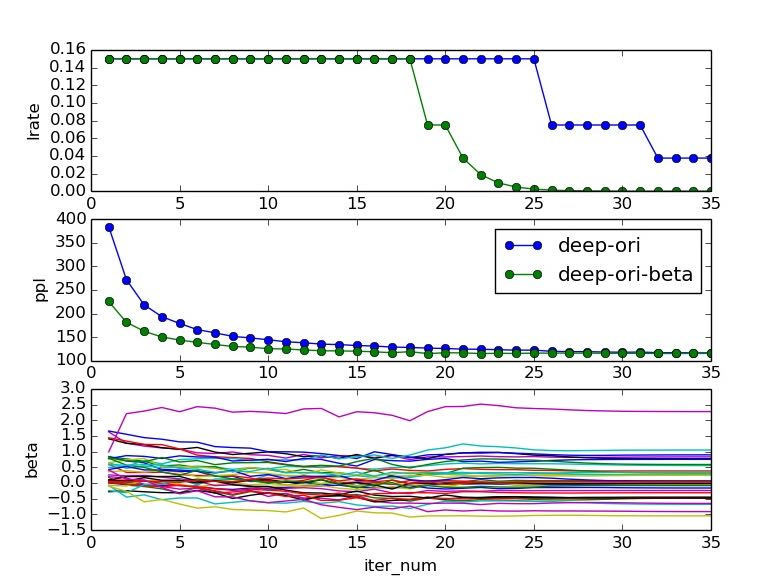
\includegraphics[width=1.5in]{exp/beta1.jpeg} 
    } 	
    \subfigure[house]{ 
        %\label{fig:subfig:a} %% label for first subfigure 
        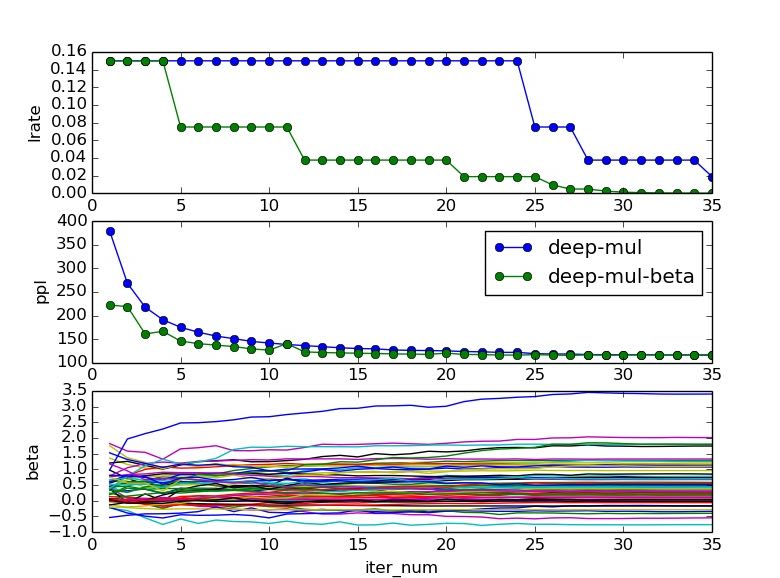
\includegraphics[width=1.5in]{exp/beta2.jpeg} 
    } 	
    \bicaption[fig:asr]{学习率、ppl和$\beta$随着轮数的变化曲线图}{学习率、ppl和$\beta$随着轮数的变化曲线图}{Fig}{The change curve of learning rate, PPL and $\beta$}
  \end{minipage}     
\end{figure}


\begin{figure}[!htbp]
  \centering
  \begin{minipage}[b]{0.6\textwidth}
    \captionstyle{\centering}
    \centering
        \subfigure[house]{ 
        %\label{fig:subfig:a} %% label for first subfigure 
        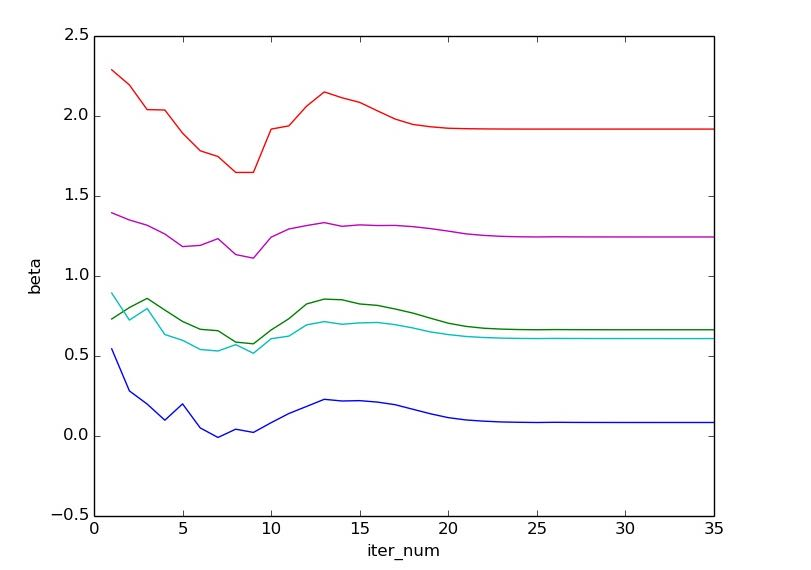
\includegraphics[width=1.5in]{exp/beta3.jpeg} 
    } 	
    \subfigure[house]{ 
        %\label{fig:subfig:a} %% label for first subfigure 
        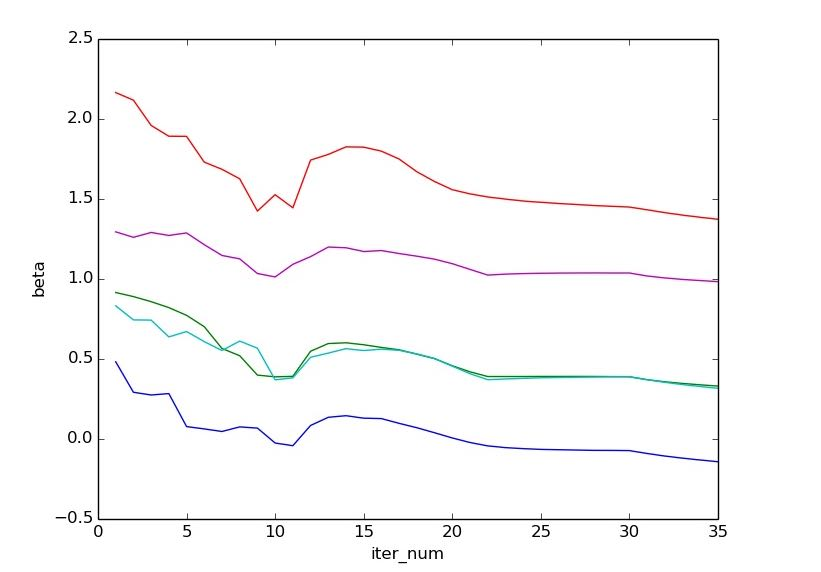
\includegraphics[width=1.5in]{exp/beta4.jpeg} 
    } 
    \bicaption[fig:asr]{beta变化曲线图}{beta变化曲线图}{Fig}{The change curve of $\beta$}
  \end{minipage}     
\end{figure}

通过这两组对比实验,我们可以更直观的发现,加入稳定算子beta的模型,ppl会更快速地收敛,以至于学习率下降得更快,到了一定范围内学习率几乎接近于$0$以至于后面的训练几乎不起作用,从而被不加稳定算子的模型接近甚至超越。另外,通过横向对比我们发现,多任务学习的PPL和学习率的收敛速度比单任务语言模型快,并且收敛后的$\beta$的绝对值要更大。
	为了探究加入稳定算子的L2范数是否能够提升语言模型,我们设计第三组实验,同样是在PTB数据上,我们控制对照组的模型结构和参数相同,一组加入原始的$\beta$,另一组在第一组的基础上加上$\beta$的L2范数。实验结果如表\ref{tab:beta3}。
    

\begin{table}[!hpb]
  \centering
  \bicaption[tab:beta3]{加入$\beta-L2norm$的比较}{加入$\beta-L2norm$的比较}{Table}{Comparison with $\beta$ or not}
   \begin{tabular}{ c| c  c | c}
            \hline
            网络类型 &
            隐层参数 &
            是否加入$\beta$和L2norm &
            PPL \\
           \hline
			LM&1lstm&None&103.346\\
			LM&1lstm&Only $\beta$&107.316\\
			LM&1lstm&$\beta$+L2norm&104.755\\
			Multitask&1lstm&None&102.207\\
			Multitask&1lstm&Only $\beta$&106.101\\
			Multitask&1lstm&$\beta$+L2norm&103.115\\
			LM&1 lstm+2 dnn&None&111.8\\
			LM&1 lstm+2 dnn&Only $\beta$&111.2\\
			LM&1 lstm+2 dnn&$\beta$+L2norm&110.1\\
			Multitask&1 lstm+2 dnn&None&110.6\\
			Multitask&1 lstm+2 dnn&Only $\beta$&110.1\\
			Multitask&1 lstm+2 dnn&$\beta$+L2norm&109.0\\
            \hline
          \end{tabular}
\end{table}
\footnotetext


如表3所示,在代码实现过程中加入$\beta$的L2范数优化后,语言模型的PPL结果有微小提升,大概1%,符合实验预期。将每个门的beta参数的根据每轮训练的变化打印如图2,可以发现加入L2范数的beta参数更小,符合上面beta越小会使PPL结果更好的猜想。




\section{实验结果与分析:面向ASR的单向辅助信息Multi-view语言模型}


\subsection{标注模型的测试与评估}

POS, NER and CHUNK是本模型主要用到的三种不同的标注.

表\ref{tab:tagging} 展示了单向LSTM标注模型在所有数据集上对三种标注的正确率。
我们对于这些标注模型的训练数据的标注并不是真实标注,这些标注来源于斯坦福大学开发的NLPCore工具进行的标注,但是在这里我们将这些标注当成是真实标注。
因此也可以说这些正确率是相比于斯坦福NLP工具的标注的相似度,甚至说相似度更为贴切。

对于这三种标注来说,可以发现正确率都不低,这也意味着使用单向模型并不会丢失太多的信息。这是在句子都是合理的情况下,当重打分任务重句子不合理的情况,相似度没有这么高,但是单向模型反而会比双向模型的标注更为合理,因为它没有使用后文不合理的信息。


    \begin{table}[th]
    \caption{\label{tab:tagging} {\it Accuracy of word-level features on all data-sets we used }}
        \centerline{
          \begin{tabular}{ c| c c c}
            \hline
            \multirow{2}{*}{Data} &
            \multicolumn{3}{c}{Accuracy(decoding/no decoding)} \\
            & POS &  NER & CHUNK \\
           \hline
            ptb& 96.36/96.32 & 80.32/82.06& 84.23/81.77\\
 %           \hline
            fisher& 94.24/94.24& 79.93/81.97& 85.72/83.47\\
 %           \hline
            sms& 94.87/94.84&80.44/82.12 & 85.55/82.98 \\
            \hline
          \end{tabular}
        }
      \end{table}

\subsection{Evaluation of training methods}
表\ref{tab:train-method} 展示了五种不同的训练方式去训练模型的PPL的区别,这五种方式在第三章提到过。对比这五种方式我们用的是sms短信数据集。

    \begin{table}[th]
    \caption{\label{tab:train-method} {\it Perplexity comparison of  different methods for training proposed model}}
        \centerline{
          \begin{tabular}{ c  c  c  }
            \hline
            {Model} &
            {Training Method} &
            {PPL} \\
            \hline
            LSTM LM& - &102.11  \\
            \hline
            \multirow{5}{*}{Multi-view LM} & 1 & 98.02  \\
%            \hline
            & 2 & 135.72 \\
            & 3 & 148.65 \\
            & 4 & 105.47 \\
            & 5 & 107.21 \\
%            \hline
            \hline
          \end{tabular}
        }
      \end{table}

实验的结果如表\ref{tab:train-method},表明第一种方式是对于单向辅助信息Multi-view语言模型来说最优的方式。第二种和第三种方法明显比第一个方法差,因为语言模型和标记模型相对独立,是两个不同的任务。将两个模型串联在一起,并对它们进行相同的学习速进行训练,将无法对两者进行适当的学习,往往会使标注模型的学习率不合适,因此不会产生双赢的结果。这一结论得到了第四和第五种方法的实验结果的支持。在使用能调节不同LSTM中学习速率的稳定算子时,PPL将远远小于第二和第三种方法。

然而,最后两种方法并没有如预期的那样超过第一个方法,因为$\beta$稳定算子只能弥补不完善的学习速率的不足,不会比用自己适当的学习速度训练它们更好。此外,第一种方法中还进行了Viterbi解码,这对于标注的合理性来说具有相当大的约束,比相比于斯坦福模型的一致性来说更重要。因为在ASR重打分任务的$n$-best句子往往不是那么合理,因此使用斯坦福的标注工具得到的标注会有很多是不准确的(即使我们将其当作标注模型的真实标注),而单向标注模型的信息抽象能力,结合Viterbi解码的约束,使得单向标注模型和斯坦福标注的准确性(一致性)不高,却经常出现斯坦福标注不合理而单向标注模型的输出更合理的情况。

这个方法看似简单,却并不是没有意义的,因为不进行这个比较实验就无法得到最好的训练方式,也不利于之后的实验分析。

因此,采用第一种方法将会被用来对所有的单向辅助信息的Multi-view语言模型进行训练。在后续的所有实验过程中,将对标注模型进行独立训练,通过Viterbi解码,然后与LSTM语言模型连接在一起。


\subsection{Multi-view语言模型的测试}

在本节中,我们使用上述数据集来评估我们的多视角语言模型的有效性。
首先,我们在PTB数据集上尝试了各种各样的模型,并将它们各自的PPL进行了比较,但是需要注意到PTB集合不支持ASR重打分任务。


如图\ref{tab:ptb}所示,对于多视角(Multi-view)语言模型来说,无论是使用斯坦福工具标注的,或者是使用我们的模型,对于PPL来说都提升非常多。其中以词性标注的提升最为巨大,大概有$10\%$。


    \begin{table}[th]
    \caption{\label{tab:ptb} {\it Perplexity comparison of different LMs on PTB data set}}
        \centerline{
          \begin{tabular}{ c c c }
            \hline
            {Model} &
            {Tagging} &
            {PPL}  \\
            \hline
            4-gram& - & 141.46 \\
            LSTM LM& -&98.73\\
            Multi-task+POS & - & 100.88 \\
            Multi-view+Multi-task+POS & - & 93.47 \\
             \hline
            \multirow{3}{*}{Multi-view+POS}
            & Standford & \underline{91.69} \\
            & \textbf{LSTM} & \textbf{93.82} \\
            \hline
            \multirow{2}{*}{Multi-view+NER}
            & Standford & \underline{97.63} \\
            & \textbf{LSTM} &\textbf{97.92}  \\
            \hline
            \multirow{2}{*}{Multi-view+CHUNK}
            & Standford & \underline{94.34} \\
          	&\textbf{LSTM}& \textbf{95.63} \\
            \hline
          \end{tabular}
        }
      \end{table}

表\ref{tab:sms} 展示了混淆度,词错误率,和句子错误率在SMS短信数据集加入不同的标注上的表现。
结果表示在加入词性标注的情况下,语言模型会有非常大的提升,命名实体和语法块的加入也使语言模型有所提升,但是提升不是很大。
主要原因可能是命名实体标注是很稀疏的标注,导致了绝大部分词的标注都是空,添加的信息不够丰富。
而对于语法块来说,标注工具的准确性并不高。
基于以上的观点,为了后续实验更加容易,我们后面仅仅在加入词性标注的额外信息基础上进行,在比较大的Swb-fisher上进行测试。

表\ref{tab:fisher}展示了混淆度,词错误率,和句子错误率在Swb-fisher数据集上加入不同的标注上的表现。这组数据的观察结果与中文短信的数据集的结果相似。
    \begin{table}[th]
    \newcommand{\tabincell}[2]{\begin{tabular}{@{}#1@{}}#2\end{tabular}}
    \caption{\label{tab:sms} {\it Perplexity, WER (\%) and SER (\%) comparison on Chinese SMS task}}
        \centerline{
          \begin{tabular}{ c  c  c  c  c }
            \hline
            {Model} &
            {Tagging} &
            {PPL} &%\multicolumn{1}{|c||}{AM} &
            {WER} &
            {SER}  \\
			\hline
            4-gram& - &124.23 & 13.41 & 42.16 \\
            %LSTM LM& - &\underline{102.11} & \underline{11.30} & \underline{41.59} \\
            LSTM & - &102.11 & 11.30 & 41.59 \\
            Multi-task+POS& - &103.42 & 11.32 & 41.63 \\
            Multi-task+Multi-view+POS& - &98.24 & 10.91 & 40.89 \\
            \hline
            \multirow{2}{*}{Multi-view+POS}
            & Standford & \underline{94.41} &11.19 & 41.92 \\
            & \textbf{LSTM} &\textbf{98.02}&\textbf{10.83}&\textbf{40.71} \\
            \hline
            \multirow{2}{*}{Multi-view+NER}
            & Standford & \underline{101.88}  & 11.28 & 41.59 \\
            & \textbf{LSTM} &\textbf{ 102.08}&\textbf{11.32}&\textbf{41.72} \\
            \hline
            \multirow{2}{*}{Multi-view+CHUNK}
            & Standford & \underline{96.71}&11.25& 41.63\\
            & \textbf{LSTM} &\textbf{100.30}&\textbf{11.02}&\textbf{41.23} \\
            \hline
          \end{tabular}
        }
      \end{table}



    \begin{table}[th]
    \caption{\label{tab:fisher} {\it Perplexity, WER (\%) and SER (\%) comparison on English Fisher task}}
        \centerline{
          \begin{tabular}{ c  c  c  c  c }
            \hline
            {Model} &
            {Tagging} &
            {PPL} &%\multicolumn{1}{|c||}{AM} &
            {WER} &
            {SER}  \\
           \hline
            4-gram&-& 79.12 & 16.3  & 53.75  \\
            %LSTM LM&-& \underline{65.42} & \underline{15.6} & \underline{53.42} \\
            LSTM &-& 65.42 & 15.62 & 53.42\\
             Multi-task+POS & - &65.93 & 15.60 & 53.65 \\
            Multi-task+Multi-view+POS& - &92.77 & 15.20 & 52.23 \\
            \hline
            \multirow{2}{*}{Multi-view+POS}
            & Standford &\underline{60.24} & 15.73 & 53.40	 \\
            & \textbf{LSTM} &\textbf{62.71} &\textbf{15.01}  &\textbf{52.19} \\
            \hline
          \end{tabular}
        }
      \end{table}


我们将本文提出的单向辅助信息LSTM语言模型和实验基线(普通传统的LSTM语言模型)相比,混淆度、词错误率和句子错误率分别减少了$4.0\%$,  $4.0\%$, $2.0\%$,无论是在中文数据集还是英文数据集上。
另外,我们的模型相比于普通的Multi-view多视角语言模型来说,在加入词性标注辅助信息时,词错误率和女字错误率上分别也减少了 $4.4\%$,  $2.2\%$ and  $3.2\%$, $2.8\%$ .

在这里需要强调的是,虽然我们的模型在混淆度这个维度上,在加入词性标注的情况下没有比普通的多视角语言模型好,但这是正常的,在面第一章和第三章的研究动机反复提到过的因为普通的多视角语言模型会引入不应该被加入的额外过多的后文信息导致混淆度很好但是在语音识别上没有提升。


对于所有的数据集,Stanford和LSTM标注模型的多视图LSTM语言模型,与LSTM RNN语言模型相比,在困惑方面有了显著的改进。
与斯坦福词性标注的普通多视角LSTM语言模型在混淆度上的结果更好,这在之前的工作中得到了广泛的验证,但在ASR重打分任务中没有显示出相应提升\cite{shi2015integrating}。

斯坦福大学的CoreNLP POS标记工具使用了最大熵算法模型\cite{Toutanova2000Enriching},利用未来的信息,未来的信息只对PPL任务有贡献,而不是ASR重打分任务。
最大熵模型使用上下文未来信息来计算文本的后验概率。
也就是说,在语言模型训练中添加这个词性标注信息,就等于将未来的信息添加到现在的单词中。这导致了一种对于混淆度的理所当然的优化,但在重新分析任务中没有WER和SER的减少。


另外,我们想确认词性标注部分是否对PPL有贡献,因此添加了另一个对比实验来验证我们的结论。为了比较所提出的和传统模型之间的标注信息的影响,我们通过对模型的输入进行删除和添加标记特性来进行实验。
%We used the language model without POS tagging, when we tested our multi-view LM, we set the output of tagging LSTM in our model to zero, which equals to removing the features of the test-data for common multi-view LM.

The comparison is shown in Table~\ref{tab:try-test}. "Without-tag" means that we deliberately remove the feature feed from the trained tagging part of proposed model. The results indicate that tests with tag feature are generally better than those without. And the latter even does not outperform an ordinary LSTM LM, which means tag feature plays an important role in the LM performance. Furthermore, the result confirms the contribution of our POS tagging model. Moreover, our model performs better than the original multi-view LM without tags, which confirms the contribution of our tagging model in the proposed multi-view structure.
该比较显示在表\ref{tab:try-test}中。“without-tag”指的是我们故意从被训练的标签部分中删除该特性。结果表明,带有标记特征的测试通常比无标记的测试更好。后者甚至没有超过普通的LSTM LM,这意味着标记特性在LM性能中起着重要的作用。此外,结果证实了我们的POS标记模型的贡献。此外,我们的模型比原始的多视图LM模型表现得更好,这也证实了我们的标签模型在多视图结构中的贡献。

   \begin{table}[th]
    \newcommand{\tabincell}[2]{\begin{tabular}{@{}#1@{}}#2\end{tabular}}
    \caption{\label{tab:try-test} {\it Perplexity on different test-data}}
        \centerline{
          \begin{tabular}{ c  c  c  c }
            \hline
            \multirow{2}{*}{Data-set} &
            \multirow{2}{*}{Tagging} &
            \multicolumn{2}{c}{PPL} \\
            & &  without-tag & with-tag \\
            \hline
            \multirow{2}{*}{PTB}
            &Standford& 98.77  & 91.69  \\
            &LSTM& 98.64  & 93.82  \\
            \hline
            \multirow{2}{*}{Fisher}
            &Standford& 66.25 & 60.24  \\
            &LSTM&65.79& 62.71  \\
            \hline
            \multirow{2}{*}{SMS}
            &Standford& 102.20 & 94.41  \\
            &LSTM&  102.13 & 98.02 \\
            \hline
          \end{tabular}
        }
      \end{table}


The proposed LSTM LM with word-synchronized auxiliary feature, performs better not only on ASR-rescore task but also PPL task.
For this result, we consider the following two aspects.
On one hand, the tagging model change the contextual information to word-synchronized auxiliary information, which is rather useful in ASR-rescore task.
On the other hand, the proposed LM with unidirectional tagging process permits the decoding of LVCSR to proceed in real time.
该LSTM LM系统具有文字同步辅助功能,不仅在asr - rescore任务上表现更好,而且在PPL任务中表现更好。
为此,我们考虑以下两个方面。
一方面,标记模型将上下文信息更改为单词同步辅助信息,这在asr - rescore任务中非常有用。
另一方面,所提出的具有单向标记过程的LM系统允许对LVCSR进行实时解码。




In this paper, we propose a multi-view LSTM LM with unidirectional tagging model, which produces word-synchronized auxiliary feature that only incorporate previous contextual information.
This auxiliary feature is combined with the word sequence to train a multi-view LSTM LM.
Five different training methods for this model are tested,
and the best one is used in the large-scale ASR task. 
In the comparison experiments between our model and related works (N-gram LM, multi-task LM, multi-view LM with Stanford tagging and multi-task combined with multi-view LM), the used data sets are PTB, English Fisher and  Chinese SMS and PPL, WER and SER are used as the evaluation criteria.
Our proposed model shows significant improvements for all word-level features including POS, NER and chunking on WER and SER.
Especially for the POS feature on English Fisher,  our proposed model not only gives gian ($4.0\%$) on PPL, but also shows significant WER and SER reduction (relative $4.0\%$ and $2.0\%$) in ASR task, compared with the baseline (LSTM LM).
Most importantly, comparing to the multi-view LM with POS feature produced by traditional model (Stanford tool), our model shows better result of WER and SER ($4.4\%$ and $2.2\%$) in ASR-rescore task. 
%Attention that the negative consequence on PPL is reasonable and it was explained in the body.
For more related models like multi-task and multi-task combined with multi-view models, our model all shows achievement in varying degrees.
%As our multi-view model performs well on the large scale ASR rescore, it is worthy to be applied in speech recognition.

